%!TEX root = ../../../super_main.tex

\section{Server Issues}
\label{sec:server_issues}

The reader is invited to reference \figref{fig:bonefire} while reading through this section. This is a timeline illustrating the events happened in the period with server-issues. 

\begin{figure}[!htbp]
	\centering
	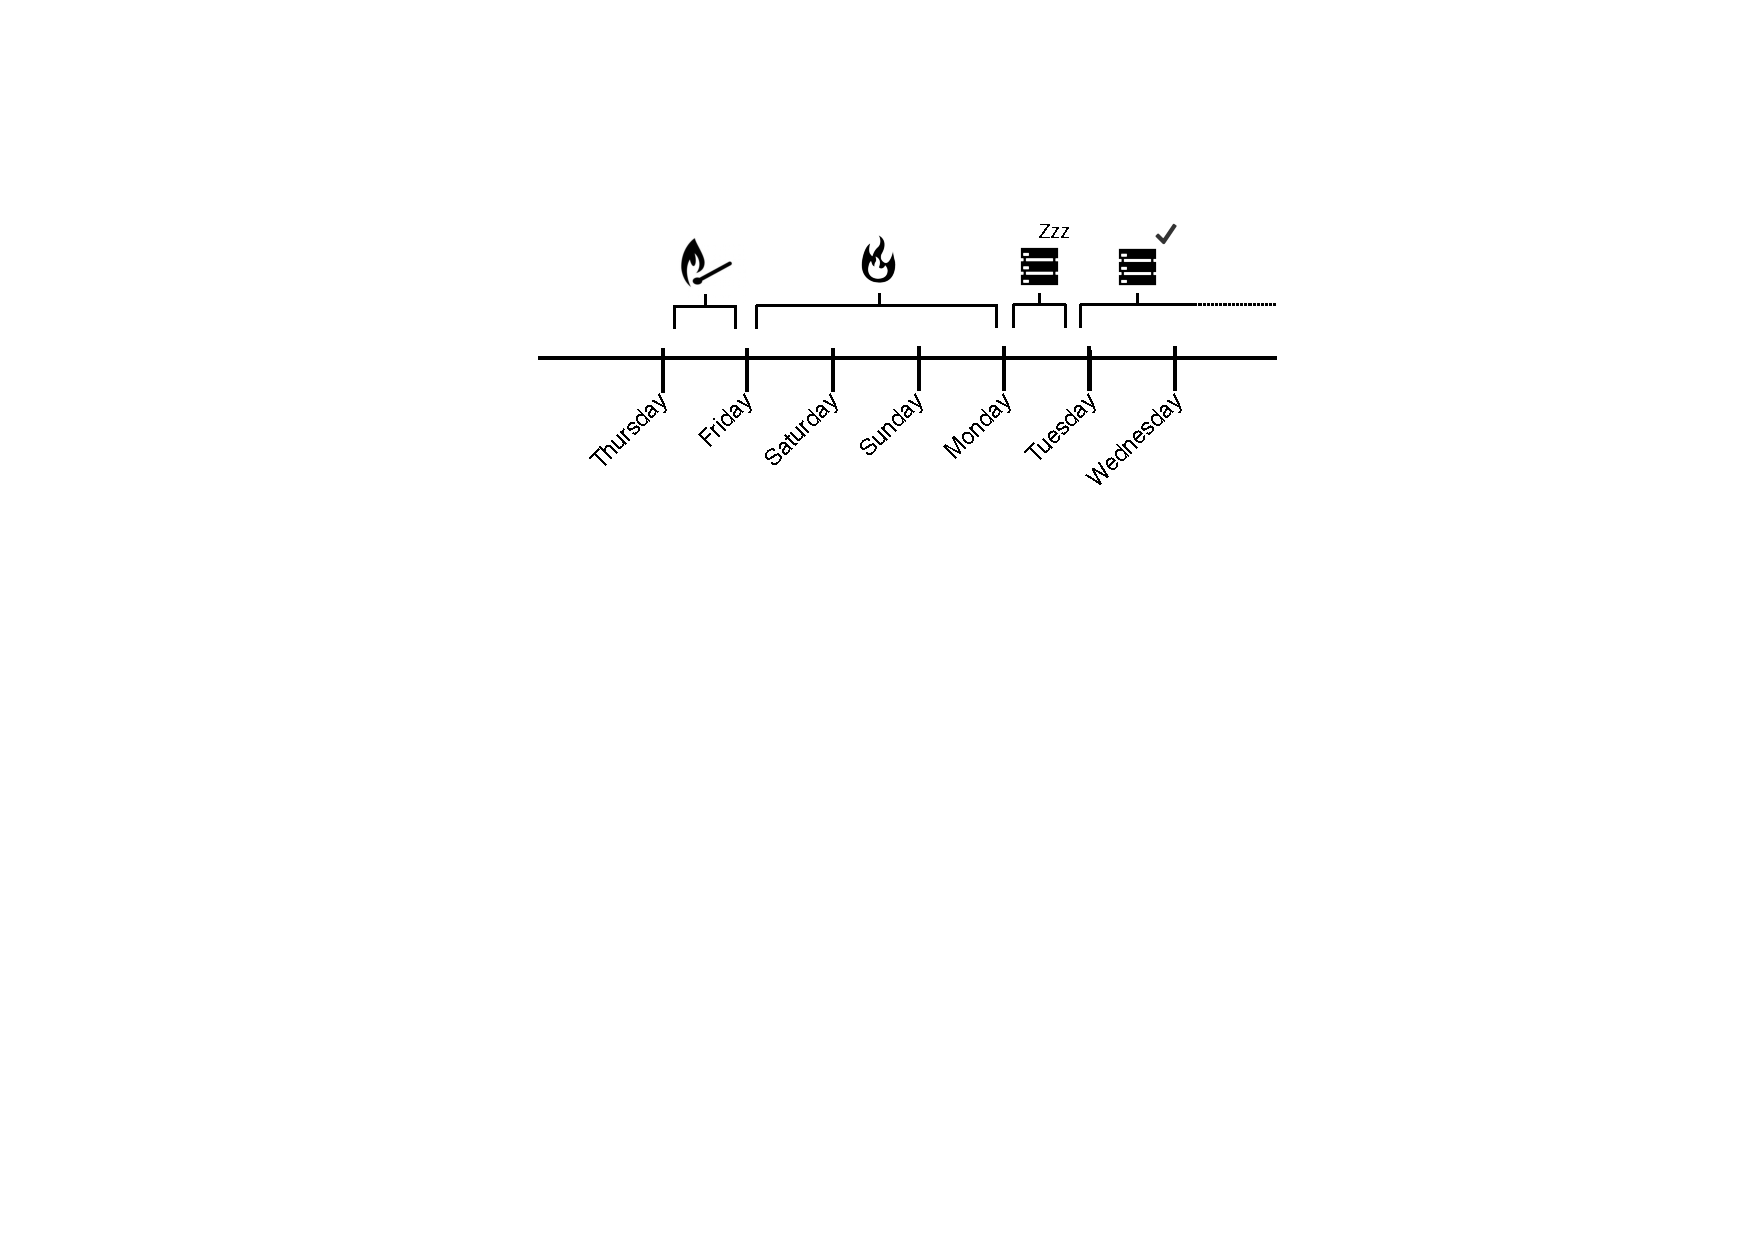
\includegraphics[width=0.75\textwidth]{bonfire}
	\caption{Timeline for the server issues}
	\label{fig:bonefire}
\end{figure}

Nearing the end of sprint four, one of the \emph{Build and Deployment} groups decided to upgrade the server with additional storage. This was attempted the night between Thursday and Friday before the planned sprint end the Wednesday after, i.e. we had five days (three actual work days and two weekend days) in between these two dates. This storage upgrade caused the entire server to crash due to some partitioning issues they had introduced. The group responsible for the update worked Friday, the entire weekend and a few hours Monday on restoring the server to a working state. Once the server worked again, the server had been rolled back to its state around 1$\frac{1}{2}$ weeks earlier, which meant that mismatches were introduced between the Git repositories located on the server and the Git repositories located on the developers' computers. 
\\\\
\todo[inline]{DONE-start (mathias) skriv at vi skulle finde udviklerne således at vi kunne få dem til at bygge i den rigtigte rækkefølge pga dependencies}
This resulted in having to push the different repositories to the git server again, and let it be known that this was no simple task. In order to maintain the dependencies and version numbering, we first had to sort out all dependencies between every project. Afterwards we had to locate the developers with the newest editions of the various repositories, such that we were sure that no code was lost during this process. When these people had been located, we had to make sure that the pushes were initiated in the correct order, starting from the deepest nested library, such that the development environment could be restored to its previous state correctly.

This process was started Monday afternoon around 15:00, which is also the final obligatory working hour across the project. Therefore some people had gone home, and one library did therefore not have its newest edition uploaded to the server. This created some issues in the system which were impossible to know the cause of, since we could not possibly know that one developer had local changes that were not on the server. Our group therefore spent the entire Monday tracking down people who had information about the following issues:
\todo[inline]{DONE-end}


\begin{enumerate}
    \item Download from remote server would not start on any client side application.
    \item Unable to login due to a ``The database does not contain any profiles'' error.
    \begin{itemize}
        \item Note: Issue 2 was revealed once issue 1 had been resolved
    \end{itemize}
    \item Unable to start applications from the \launcher  
    \begin{itemize}
        \item Note: Issue 3 was revealed once issue 2 had been resolved
    \end{itemize}
\end{enumerate}


Issue 1 was related to rolling back the MySQL server, which had created a mismatch between the MySQL user password located on the Jenkins server and the actual password needed to access the database. This was resolved due to help from group \emph{SW610F15}, whom suggested changing the MySQL password to a previous version.
\\\\
Once issue 1 had been resolved, issue 2 presented itself when trying to log into the \giraf \launcher. No matter how one attempted to login, an Android Toast (small message) would be displayed saying that no profiles were present in the database. This issue was directly related to one of the groups not pushing all their work after the server reset. This group had been working on making some applications standalone, and therefore also worked on a standalone \androidinline{ContentProvider}. A \androidinline{ContentProvider} is used in Android applications to manage access to a data source \parencite{android_content_provider}. 
\\\\
The \androidinline{ContentProvider} used by the standalone applications would change from the \androidinline{ContentProvider} provided by the \launcher to the application's own standalone \androidinline{ContentProvider}. The paths to the content provider they should use, is found in a file called \mono{QuxContentProviderAuthority.java}.
\\\\
This new way of managing content providers, unfortunately had the side effect, that the \launcher also had to have a file called \mono{QuxContentProviderAuthority.java} which had to reference its own content provider in order to make the \launcher work properly. The issue then was, that the \launcher did not have such a file, since the group working on standalone applications had not informed anyone else about how this new system worked, and the file committed by the standalone group had not been added to the \launcher repository after the rollback. 
\\\\
The effect of this missing file was that any SQL calls would just return that the size of any accessed table was zero, even though it was clearly visible through the log in Android Studio that all data was downloaded with the initial download. Once this had been discovered, the missing \mono{QuxContentProviderAuthority.java} file was added to the launcher and the login functionality was once again working.
\\\\
Hereafter it was discovered that all the other applications were getting the same error as in issue 2, once attempted launched through the \launcher application (issue 3). This was caused by a coding mistake in the \emph{Meta-Database} repository which contains the implementation of how to handle the content providers mentioned in issue 2. The implementation did not correctly check whether or not applications were launched from the \launcher, which caused every application to have to contain the \mono{QuxContentProviderAuthority.java} as well, which was not intended by the group who worked on the content providers. To solve the issue we included the Qux file in every application, and we could finally correctly start all the applications come Tuesday around 17:00. 
\\\\
We managed to solve all three issues, such that all applications in the \giraf suite was in a usable state, and we could therefore successfully execute the Sprint Review Meeting with customers present without any issues or crashes. Furthermore the group which had introduced issue 2 and 3 were aware of the mistake, and implemented a fix by Wednesday afternoon such that only the standalone applications and the \launcher were required to have the \mono{QuxContentProviderAuthority.java} file when updated to new versions of their libraries.
\\\\
Even though we managed to solve the issues after the server crash, the consequences was that there was spent a lot of time on resolving an issue rather than spending time on resolving other development tasks. Since this problem occurred so close to the end of the sprint, some groups were forced to extend the workdays to reach the goal of stable and polished applications.
